\question
В перерыве между парами дискретной математики вы с друзьями решили зарубиться в домино. Иллюстрация ниже визуализирует данный момент игры.

\\
\begin{figure}[h]

\begin{minipage}[h]{0.55\linewidth}
\end{minipage}
\begin{minipage}[h]{0.45\linewidth}
\center{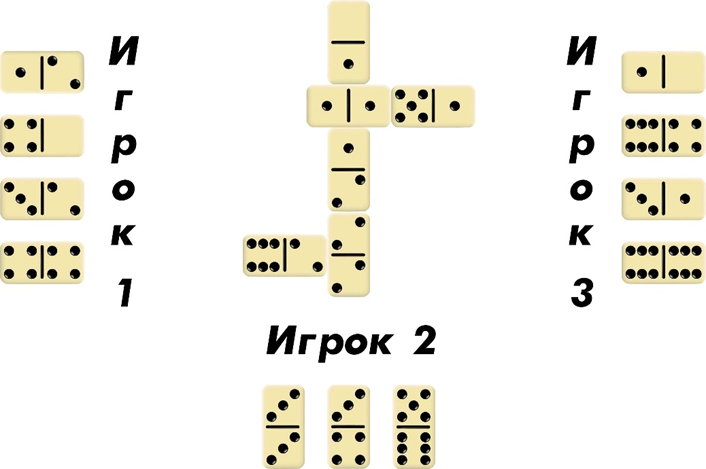
\includegraphics[width=0.7\textwidth]{pic/941.png} }
\end{minipage}
\end{figure}

Так как вы — умные студенты, вам стало интересно интерпретировать партию в виде бинарных отношений. Запишите отношения:
\begin{itemize}
    \item $G = \{(a,b)|a$ и $b$ – стороны свободных доминошек, лежащих на столе, где a – свободная сторона$\}$
    \item $R_1 = \{(a,b)|a$ и $b$ – стороны одной доминошки в руке у первого игрока$\}$
    \item $R_2 = \{(a,b)|a$ и $b$ – стороны одной доминошки в руке у второго игрока$\}$
    \item $R_3 = \{(a,b)|a$ и $b$ – стороны одной доминошки в руке у третьего игрока$\}$
\end{itemize}

Используя операцию композиции, составьте новые бинарные отношения:
\begin{itemize}
    \item $P_1$ – возможные ходы у первого игрока
    \item $P_2$ – возможные ходы у второго игрока
    \item $P_3$ – возможные ходы у третьего игрока
\end{itemize}


Ходом является пара крайних номеров стоящих рядом доминошек.
\\
---------------

Автор -- Константин Васильев, М3213